\documentclass[12pt]{article}
\setlength{\headheight}{14pt}

% 杂项宏包
\usepackage[colorlinks,linkcolor=blue]{hyperref}  % 超链接
\usepackage{amsmath}
\usepackage{amssymb}
\usepackage{multicol}
\usepackage{indentfirst}
\usepackage{algorithm}   % 代码块
\usepackage{algorithmicx}   % 代码块
\usepackage{algpseudocode}   % 代码块 
\usepackage{graphicx}  % 图片
\usepackage{subfigure}  % 并排图像
\usepackage{fontspec}
%\usepackage{parskip}
\usepackage[]{caption2}  % 去掉图表的冒号
\renewcommand{\captionlabeldelim}{}  % 去掉图表的冒号
\usepackage{booktabs} % 三线表
\usepackage{pdfpages}  % 直接插入pdf页面
% \setlength{\parindent}{2em}

% 字体设置
\usepackage{xeCJK}
%%%%%%%%%%% CJK下设置中文字体 %%%%%%%%%%%%%
\setCJKmainfont{SimSun.ttf}  % 中文字体
\setCJKsansfont{simhei.ttf}
\setCJKmonofont{simkai.ttf}
\setCJKfamilyfont{song}{SimSun.ttf}
\newcommand{\song}{\CJKfamily{song}}
\setCJKfamilyfont{kai}{simkai.ttf}
\newcommand{\kai}{\CJKfamily{kai}}
\setCJKfamilyfont{fang}{simfang.ttf}
\newcommand{\fang}{\CJKfamily{fang}}
\setCJKfamilyfont{hei}{simhei.ttf}
\newcommand{\hei}{\CJKfamily{hei}}
\setCJKfamilyfont{li}{SIMLI.TTF}
\newcommand{\li}{\CJKfamily{li}}
\setmainfont[BoldFont=Times-Bold.ttf, ItalicFont=Times-Italic.otf]{Times.ttf}  % 英文字体
\setsansfont{Source Sans Pro}
\setmonofont{simkai.ttf}



\usepackage{gbt7714}  % 国标参考文献
\renewcommand\refname{\hei \sihao 参考文献}

% 页面布局设置
\usepackage{geometry}
\geometry{a4paper, scale=0.8}  % 页面边距
% \setlength{\parskip}{1.15em}  % 段落之间空 0.5 行


% 其他设置
%%%%%%%%%%%  设置字体大小 %%%%%%%%%%%%%
\newcommand{\chuhao}{\fontsize{42pt}{\baselineskip}\selectfont}   %%%初号字体
\newcommand{\xiaochuhao}{\fontsize{36pt}{\baselineskip}\selectfont}    %%%小初号字体
\newcommand{\yihao}{\fontsize{28pt}{\baselineskip}\selectfont}   %%%一号字体,以此类推
\newcommand{\erhao}{\fontsize{21pt}{\baselineskip}\selectfont}
\newcommand{\xiaoerhao}{\fontsize{18pt}{\baselineskip}\selectfont}
\newcommand{\sanhao}{\fontsize{15.75pt}{\baselineskip}\selectfont}
\newcommand{\sihao}{\fontsize{14pt}{\baselineskip}\selectfont}
\newcommand{\xiaosihao}{\fontsize{12pt}{\baselineskip}\selectfont}
\newcommand{\wuhao}{\fontsize{10.5pt}{\baselineskip}\selectfont}
\newcommand{\xiaowuhao}{\fontsize{9pt}{\baselineskip}\selectfont}
\newcommand{\liuhao}{\fontsize{7.875pt}{\baselineskip}\selectfont}
\newcommand{\qihao}{\fontsize{5.25pt}{\baselineskip}\selectfont}

%%%% 设置 section 属性 %%%%
\makeatletter
\renewcommand\section{\@startsection{section}{1}{\z@}%
  {-1.5ex \@plus -.5ex \@minus -.2ex}%
  {.5ex \@plus .1ex}%
  {\normalfont\sihao\fang}}  %%这边要是不想要宋体三号字,可以把song改成之前定义的字体和字号。
%{\normalfont\sihao\CJKfamily{fs}}}  %%比如改成仿宋四号,前面定义好了,后面只需要改几个字母就可以了。
\makeatother
%%%% 设置 subsection 属性 %%%%
\makeatletter
\renewcommand\subsection{\@startsection{subsection}{1}{\z@}%
	{-1.25ex \@plus -.5ex \@minus -.2ex}%
	{.4ex \@plus .1ex}%
	{\normalfont\wuhao\hei}}
\makeatother
%%%% 设置 subsubsection 属性 %%%%
\makeatletter
\renewcommand\subsubsection{\@startsection{subsubsection}{1}{\z@}%
	{-1ex \@plus -.5ex \@minus -.2ex}%
	{.3ex \@plus .1ex}%
	{\normalfont\wuhao\song}}
\makeatother
% 章节从 0 开始
\setcounter{section}{-1}

% 算法标题设置
\floatname{algorithm}{\xiaowuhao 算法}
\renewcommand{\algorithmicrequire}{\textbf{输入:}}
\renewcommand{\algorithmicensure}{\textbf{输出:}}

\renewcommand{\figurename}{\xiaowuhao \hei 图}
\renewcommand{\tablename}{\xiaowuhao \hei 表}

  % 导入配置文件

\newcommand\titleofdoc{东 南 大 学 研 究 生 课 程 论 文} % 文档标题
\newcommand\GroupName{基于深度学习的源代码错误定位研究} % 小组名

\usepackage{fancyhdr}
\pagestyle{fancy}
\fancyhf{}
\fancyhead[C]{\small 东南大学}

\setcounter{section}{0}


% 正文
%%%%%%%%%%%%%%%%%%%%%%%%%%%%%%%%%%%%%%%%%%%%%%%%%%%%%%%%%%%%%%%%%%%%%%%%%%%%%%%%%%%%%%%%%%%%%%%%%%%%%%%%%%%%%%%%%%%%%%%
\begin{document}
\begin{sloppypar}  % 两端对齐命令

    % \input{sections/cover.tex}  % 封面文件

    
\begin{center}
  \erhao \sffamily 基于机器学习的源代码错误定位研究报告

  \vspace{0.3cm}

  \xiaosihao \ttfamily 吴清晏$1$ \quad 杨锦波$2$ \quad 张闻启$3$ \quad 董子翔$4$ \quad 万奕含$5$

\end{center}

\xiaowuhao{
  \noindent \sffamily 摘要: \normalfont 在本文中,我们探讨了基于机器学习的错误定位方法,包括基于向量空间的方法、基于学习排名的方法、基于代码修改历史的方法、基于执行信息的方法,以及基于深度学习的方法。近年来深度学习模型在自然语言处理领域取得了重大突破,这将会催生出更多新的高效的静态错误定位方法。希望通过本文的介绍,能够帮助读者理解机器学习在源代码缺陷定位中的应用,为后续的研究工作提供参考。

  \noindent \sffamily 关键词:\normalfont 错误定位;错误报告;深度学习;预训练模型
}

\begin{center}
  \sihao Fault-localization based on machine learning models

  \vspace{0.3cm}

  \xiaosihao \ttfamily Qingyan Wu$^1$ \quad Jinbo Yang$^2$ \quad Wenqi Zhang$^3$ \quad Zixiang Dong$^4$ \quad Yihan Wan$^5$

  \xiaowuhao (1. Southeast University, 211189, Nanjing, China)

\end{center}
\xiaowuhao{
  \noindent \textbf{Abstract:} In this paper, we explore various fault localization methods based on machine learning, including those based on vector space models, learning to rank, code modification history, execution information, and deep learning. In recent years, deep learning models have achieved significant breakthroughs in the field of natural language processing, which will give rise to more efficient static error localization methods. Through this paper, we hope to help readers understand the application of machine learning in source code defect localization and provide a reference for subsequent research work.

  \noindent \textbf{Keywords: } fault localization; bug report; deep learning; pre-trained model
}

  % 标题及摘要文件

    \vspace{0.5cm}  % 分隔 0.5cm


    \section{引言}  % 第一个section的标题(一般为引言,此处不分栏,因为根据 word 模板来看,这一行似乎是单独的,但是内容又是要分栏的,所以把第一个section的标题和内容分开了)
    \begin{multicols*}{2}  % 正文开始分栏

        软件是现代生活的重要组成部分,当软件出现错误时,开发人员需根据错误报告的描述来定位和修复错误。然而,错误报告通常由非专业人员编写,包含大量自然语言描述,这给错误定位和修复带来了很大的困难。此前,已有一篇2016年的研究调查了20世纪70年代以来与错误定位有关的大量报告\cite{7390282},该研究全面介绍了8类错误定位方法,但没有详细介绍机器学习类方法。本文将关注基于机器学习的静态错误定位方法。
\section{名词解释}
\subsection{错误定位}
错误定位方法分为静态错误定位和动态错误定位。静态错误定位仅分析源代码,不运行程序。动态错误定位需运行程序,分析程序的执行过程和测试用例的执行结果。机器学习方法主要应用于静态错误定位方法。

错误定位常用的评估指标有累积检查语句数,错误定位代价,检查得分和时间开销等。
\subsection{信息检索}
信息检索技术属于信息科学,常用于从大量的文本数据中检索出与用户需求相关的信息。基于信息检索的错误定位技术是最常见的静态错误定位方法,常被用于从错误报告中检索出与错误相关的代码片段。基于信息检索的错误定位方法主要包括以下几个步骤:
\begin{enumerate}
    \item 语料库创建:对源代码进行词法分析,去除程序关键词,分词并去除停用词,将处理后的代码片段存储在数据库中。
    \item 索引:构建单词与文件之间的索引,以便快速检索。
    \item 查询构建:处理错误报告,提取关键词,构建查询。
    \item 检索和排名:计算查询与语料库中代码片段的相似度,对代码片段进行排名。
\end{enumerate}

错误定位常用的指标大部分依赖累积检查语句数,但基于信息检索的错误定位方法必须检查所有的代码行,累积检查语句数是一个固定值,无法通过改进算法来减少。因此,通常会采用信息检索领域的评估指标,如Top K,Mean Average Precision(MAP)和Mean Reciprocal Rank(MRR)等。
\subsection{机器学习}
机器学习分为基于神经网络的方法和基于传统机器学习方法。基于神经网络的方法包括卷积神经网络(CNN),循环神经网络(RNN)等。基于传统机器学习方法包括支持向量机(SVM)和决策树等。机器学习方法的步骤如下:
\begin{enumerate}
    \item 特征提取:将源代码转换为特征向量。
    \item 数据集划分:将数据集划分为训练集和测试集。
    \item 模型训练:使用训练集训练模型。
    \item 模型评估:使用测试集评估模型。
\end{enumerate}

从2020年开始,Transformer结构的模型开始成为机器学习的主流,如BERT,GPT等。这些模型在自然语言处理领域取得了巨大的成功,也被应用于错误定位领域。

采用预训练模型的方法通常会先在大规模数据集上进行预训练,再在特定任务上进行微调。这种方法可以提高模型的泛化能力,减少过拟合的风险。其步骤与机器学习方法有一定的区别:
\begin{enumerate}
    \item 预训练:在大规模数据集上进行预训练。
    \item 微调:在特定任务上进行微调。
    \item 模型评估:使用测试集评估模型。
    \item 模型解释:解释模型的预测结果。
\end{enumerate}
\section{论文统计}
为了探索机器学习技术在静态错误定位领域的应用历史,我们通过在IEEE,ACM,Science Direct和Springer上搜索fault localization和机器学习类关键词,找到了从2013到2024的100篇论文:
\begin{figure}[H]
    \centering
    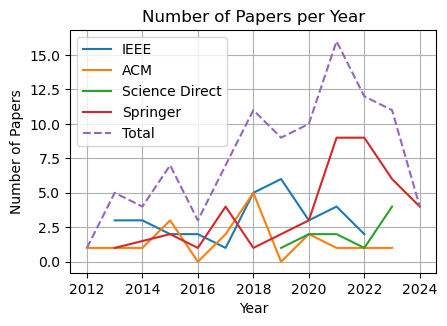
\includegraphics[width=3in]{sections/figs/articles.png}
    \caption{\label{fig1111} \xiaowuhao \hei 论文统计}
\end{figure}

可以看到,2013年静态错误定位方法开始出现,2015年达到第一个高峰,2018年达到第二个高峰,2019年开始论文增长迅速,但近两年数量有所下降。这说明,机器学习技术在错误定位领域的应用逐渐成熟,且有较大的发展空间。
  % 第一个section的内容,接上面的标题

        \section{基于向量空间的方法}
Buglocator\cite{6227210}使用向量空间模型(rVSM)根据bug报告和源代码之间的文本相似性对所有文件进行排名,同时考虑之前已修复的相似bug的信息。

同一时期的BLUiR\cite{6693093}充分利用了代码结构信息,引入抽象语法树(AST)以保存更多的结构信息,同时丢弃了语言标识符,让模型能在保留代码结构信息的同时关注语句间关联。

后续研究开始将以上思路拓展到其他错误定位任务中,如Sahu等\cite{6976082}尝试在非面向对象的编程语言如C上使用该方法(此前研究均基于Java语言),发现Buglocator依然有效,但引入代码结构信息的效果有限。这或许表明面向对象编程语言的结构信息对错误定位更为有效。

Le等\cite{6982639}使用支持向量机(SVM)构建了一个预测模型来评估该方法的有效性。当方法如Buglocator生成的可疑度排名不可靠时,该方法可以提醒研究人员及时改用传统调试方法。

2014年,Hill等人\cite{6747185}进一步探索了邻近位置信息在静态错误定位中的应用。该方法使用马尔可夫随机场(MRF)构建依赖关系图来对检索的项间依赖关系进行建模,并使用Software Word Usage Model(SWUM)\cite{hill2010integrating}提取错误报告中的短语概念(phrasal concepts)。

2016年,MULAB\cite{7816459}将VSM扩展为MULti-ABstraction VSM以考虑多抽象级别(即同一单词在不同语境下的不同含义),并使用adaptive LDA和遗传算法(LDA-GA)来调整每个抽象级别的主题号。

2019年,Liu等\cite{8736209}的研究将词嵌入方法引入向量空间方法,这是2016年词嵌入被用于软件工程领域开始,首次将其引入错误定位。Amasaki等\cite{8906763}比较了多种向量化方法,从Buglocator使用的tf-idf方法开始,到其他tf-idf方法和Word2Vec方法。该研究采用了Bench4Bl提供的评估框架。

2021年,WEQE\cite{9700273}采用了自动查询扩展(AQE),这项技术依赖首次检索时使用的查询质量,故采用单词嵌入技术来识别初始查询中的语义关键词。
\section{基于学习排名的方法}
学习排名(Learning to Rank)是一种机器学习技术,2014年Ye等人\cite{10.1145/2635868.2635874}首次将学习排名(LR)技术引入静态错误定位,并构建了一个更大的基准数据集,后续研究往往均会根据此基准数据集评估方法有效性。此外,该方法首次使用Top K,MAP和MRR作为衡量指标,这也成为了后续方法的常用指标。LR技术在6个Java项目上的表现均超越了Buglocator。

然而,\cite{7272945}发现LR技术的效果与标准的向量空间模型(VSM)类似,且在Top k指标上更差。向量空间模型首先把代码和错误报告映射到向量空间,再计算余弦相似度,这种方法利用的信息更少且同样有效。后续研究在相关性的评估上多沿用VSM方法,但向量化的方式各不相同。
\section{基于代码修改历史的方法}
2015年开始,研究人员开始尝试使用代码修改历史来提高错误定位的效果。BLIA\cite{7467300}使用代码修改历史来改进IRFL方法,发现代码修改历史可以提高错误定位的准确性。这一发现在后续研究中得到了证实,如Locus\cite{7582764}利用错误报告与更改日志中包含的信息之间的相关性提升了基于VSM的静态错误定位方法方法的性能。

Bugpecker\cite{9286037}通过代码修订图来跟踪代码修改历史,同时采用了抽象语法树来处理代码结构信息。2021年,MRAM\cite{9462960}结合了循环神经网络(RNN),注意力模型和多层感知机(MLP),解决了原先方法无法弥合语义差距,无法充分利用历史修改信息的问题。该方法同样使用代码修订图来揭示函数间关系,且由于引入了Attention机制,可以更好地处理上下文信息。这两种方法均采用了Ye等人创建的基准数据集。
\section{基于执行信息的方法}
不断有研究尝试结合动态方法来提高静态方法的定位效果,常见的执行信息包括覆盖率、切片和频谱,\cite{7961521}把这些执行信息应用到Buglocator和BLUiR等经典的静态错误定位方法中,发现仅添加覆盖信息就大大提高了这些技术整体有效性,其中在类(class)级别对BLUiR方法的提升最为显著,而切片信息进一步提高了效果,频谱信息在函数级别显著提高了定位效果,但在类级别提升有限。
\section{基于深度学习的方法}
2017年起,人们开始思考如何更好地使用深度神经网络表示代码语言\cite{10.1145/3106237.3106290}。Chen\cite{10062428}等人采用了对抗神经网络的思想,比单一使用CNN等神经网络的方法效果更好。

2020年一篇名为《Attention is All You Need》\cite{NIPS2017_3f5ee243}的论文提出了Transformer模型,这一模型在自然语言处理领域取得了巨大成功(如Bert,GPT等自然语言模型),因为它可以更好地处理上下文语境。在这之后,Transformer开始成为深度神经网络的代名词,该技术在各方面超越了CNN,RNN等传统神经网络,在处理长文本上也有较好的效果。同样在2020年,代码搜索领域的方法开始被应用于错误定位\cite{9462960}\cite{Liang2022},因为代码搜索领域同样需要弥合自然语言和代码语言间的语义差距。

2021年,DeepFL\cite{9653844}将Transformer技术应用到错误定位中,这是第一个将该技术应用于即时行级缺陷定位任务的模型,可以做到在第一时间准确定位错误。该方法采用Seq2Seq结构,包含编码器和解码器,其输入和输出均为代码语言,输出的代码语言是更“干净”\cite{6227135}的。当输入一个包含缺陷代码的错误报告时,模型会计算每一行代码及其周围代码与“干净”代码的差距,差距即为可疑度分数。该方法是最先进的基于深度学习的错误定位方法之一,且已开放数据集。

2022年,FLIM\cite{Liang2022}借用了自然语言处理领域常见的先预训练后微调形式,采用了CodeBERT\cite{2020CodeBERT}这一预训练模型。实际上,CodeBERT已经在代码搜索领域取得了巨大成功,因为大模型可以更好地弥合自然语言和代码语言间的语义差距。FLIM同时采用了LR学习排名技术来进一步处理预训练模型的输出,生成可疑度排名。
\section{其他方法}
\cite{8973028}首次采用代码异味检测技术改进静态错误定位,该方法使用了两种成熟的技术进行结合,效果提升明显。

BoostNSift\cite{9610655}没有采用额外的信息输入,但在Buglocator的数据集上达到了Buglocator和BLUiR近3倍的性能。与Buglocator等采用的tf-idf向量化技术不同,该方法采用了更符合直觉的BM25。BM25对相关性更敏感,对较长和较短的函数有着更好的处理能力。该方法的最大特点是文本提升技术,先对错误报告和代码分别进行提升,再进行搜索。该方法如果与其他方法进行混合,可能会产生更好的效果。该方法已开放数据集,数据集包含Buglocator与Ye等人的数据集。
\section{数据集选取}
2018年,\cite{8449523}发现此前许多研究的数据集是无效的,因为这些数据集将测试文件包含在了数据集中,这可能会导致评分虚高。在去除了测试文件后,Buglocator依旧有效,但是BLUiR的MAP评分和MRR评分均明显下降,这可能意味着之前大量研究中,BLUiR方法的效果被高估了。

同一年,\cite{10.1145/3213846.3213856}反驳了上述看法,认为无须去除测试文件,并给出了一个完整的评估框架Bench4BL。后续的大量研究都采用了这个评估框架。

Rahman等\cite{10.1145/3183440.3195003}探索了数据集中错误报告的代码含量对静态错误定位方法的影响。具体来说,他们选择了采用BugZilla或JIRA错误管理系统的项目,构建了仅包含自然语言的错误报告数据集和含有大量代码描述的错误报告数据集,发现缺少代码信息和过多代码信息都会降低定位工具的性能。

Zhang等\cite{https://doi.org/10.1002/smr.2312}重点关注了深度学习数据集的平衡问题,他们认为,要学习代码的特征,需要正确和错误代码的数量达到平衡,否则模型会倾向于学习错误代码的特征。他们提出了一种重采样技术,可以改善数据集不平衡问题。  % 第二个section(标题加内容)

        \section{结束语}
本文详细回顾了基于机器学习的错误定位方法,包括基于向量空间,学习排名,代码修改历史,执行信息,深度学习,以及其他方法。我们发现,尽管这些方法在错误定位任务上取得了显著的成果,但仍然存在许多问题。例如,如何更好地利用代码的结构信息,如何有效地结合静态和动态的信息,以及如何处理大规模的代码库等。

我们期待看到更多的研究能够解决这些问题,并进一步提高错误定位的准确性和效率。深度学习是机器学习中的一种强大的工具,有很大的潜力在错误定位任务上取得更大的突破。此外,我们也期待看到更多的研究能够探索新的错误定位方法,例如,利用代码的语义信息,或者结合人类的专业知识等。  % 

        % ...后续section


        % 参考文献
        \bibliographystyle{plain}  % 参考文献的格式
        \vspace{0.5cm}
        \nocite{*}
        \bibliography{sections/refs.bib}  % 参考文献bib文件
    \end{multicols*}


\end{sloppypar}
\end{document}

%%%%%%%%%%%%%%%%%%%%%%%%%%%%%%%%%%%%%%%%%%%%%%%%%%%%%%%%%%%%%%%%%%%%%%%%%%%%%%%%%%%%%%%%%%%%%%%%%%%%%%%%%%%%%%%%%%%%%%%%%%%%%%%%%%%%%%%%%%%%%%%%%%%%%%